\section{zmq-broker2}

The message broker prototype previously described was rewritten with
the following changes:
\begin{itemize}
\item{Replaced my 0MQ wrapper library with libczmq\footnote{See
  \url{http://czmq.zeromq.org/manual:_start}}}
  for multipart message ADT.
  Previous wrappers hardwired 3-part message format, but new routing
  requires a number of envelope parts dependent on number of hops.

\item{Replaced pub/sub socket for sending messages to plugins with a per-plugin
  push/pulll socket.  Now the broker peeks inside messages to determine
  which socket to send on.  This solves the message loss problem of the
  previous prototype.}

\item{Added dealer/router socket for request routing. Local request flow is now:
\begin{verbatim}
   Req: plugin(dealer) -> cmbd(router) -> cmbd(plugin.push) -> plugin(pull)
   Rep: plugin(dealer) <- cmbd(router) <- cmbd(pull)        <- plugin(push)
\end{verbatim}
  The dealer/router sockets are bidirectional.  The Req direction blocks,
  the Rep direction drops when queues are full.  In theory this works b/c
  blocking requests rate-limit replies.}

\item{The cmbd sends NACK responses to unroutable requests
  (but not before trying to route them upstream, see below).}

\item{Ping utility modified to take a plugin destination.  Ping messages pass
  through plugin's socket queues so response time indicates queue congestion,
  or can elicit a NACK if plugin is not loaded.}

\item{Replaced ad-hoc wire protocol on UNIX domain sockets with multipart message
  serialization provided by libczmq.  Client uuids are pushed onto message
  envelope, conforming to new routing protocol.}

\item{The same cmbd router socket used by plugins now also binds to the
  reduction tree input address.  A dealer socket connects to the upstream
  node.  The reduction tree thus can be used to route requests upstream.
  In fact, all reduction messages are "requests" now, with optional replies
  possible in the reverse direction.}

\item{Unmatched requests recurse upstream instead of being NACKed locally.
  This allows services to be located anywhere in the tree, transparent to
  the API.}

\item{For the single-redis KVS configs tested before, the kvs plugin is simply
  loaded on the root node and the reduction network used to route requests.
  Before we loaded kvs plugin everywhere and pointed hiredis to the address of
  the redis running on the root node.  Latency is increased but of course
  the previous method would have fallen over when the number of sockets
  opened by the redis server exceeded the system max.}

\item{Plugins that want to insert themselves into the reduction path are
  accomodated by a new routing rule:  messages sent by a plugin to itself
  are routed upstream rather than looped back.   A plugin simply receives
  "requests" from downstream, and sends reduced "requests" upstream.
  The barrier plugin was reworked to behave this way.}

\item{Reworked liveness protocol so that only direct descendents are monitored
  and parent publishes down|up events via EPGM.  Each node listens for
  state changes and maintains a copy of the session livenesss state.}

\item{Added a 'snoop' pub/sub socket which receives all router traffic,
  so a tool can watch all the traffic being passed by the local cmbd.
  Before we just subscribed to everything on the internal pub/sub "bus",
  but that is no longer available.}

\item{Factored poll loop and receive functionality out of plugins.
  Plugins can now register init, fini, recv, and timeout functions.
  They can also override the poll function if necessary (API plugin does
  this since it needs to monitor UNIX domain sockets also).}

\item{'ping' and 'stats' request handling implemented for each plugin
  automatically in the abstracted-away poll loop.}
\end{itemize}

\begin{figure}
\centering
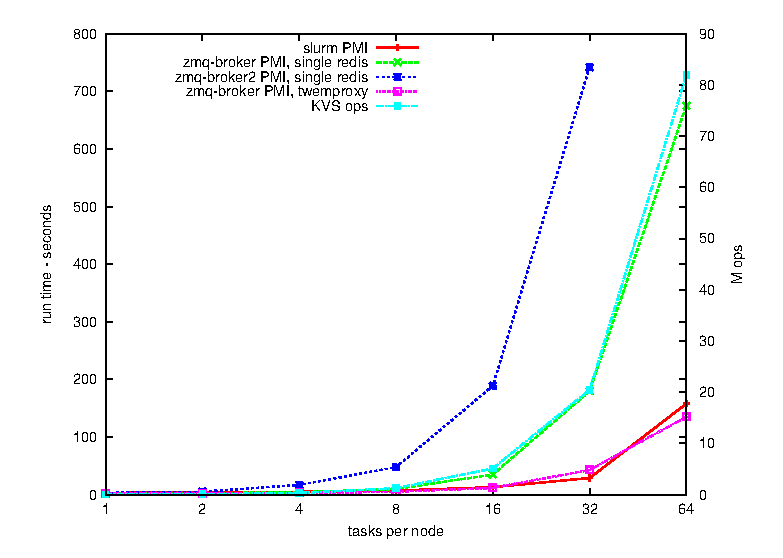
\includegraphics[scale=1.2]{zmq-broker-pmi2.eps}
\caption{Scaling of MPICH2 hello world program on 100 nodes of hype wired
in a trinary tree.  zmq-broker2 scaling is inferior to zmq-broker because
the RTT of a KVS op, now carried over multiple overlay hops,
is increased from about a flat $500\mu$s, to about $500\mu$s per hop.
Also the requests are serialized between the root KVS and redis.
However, the scalability of the number of kvs clients is greatly increased
in zmq-broker2 since the per-process socket limit is not a factor.}
\label{fig:cmb2scale}
\end{figure}

\begin{figure}
\begin{minipage}[b]{0.10\linewidth}
  \centering
  \fbox{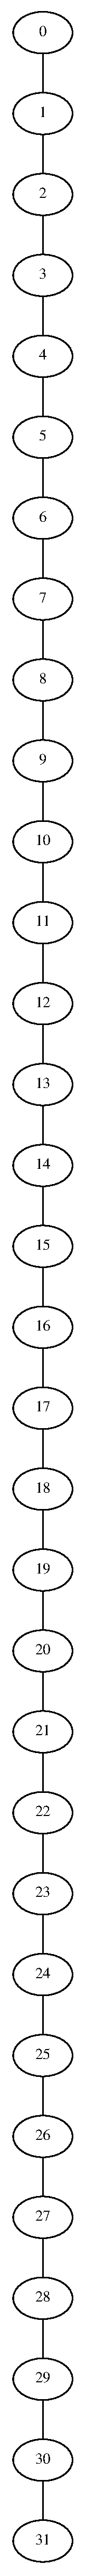
\includegraphics[scale=0.2]{tree-degenerate}}\\
  degenerate
\end{minipage}
\hspace{0.5cm}
\begin{minipage}[b]{0.80\linewidth}
  \centering
  \fbox{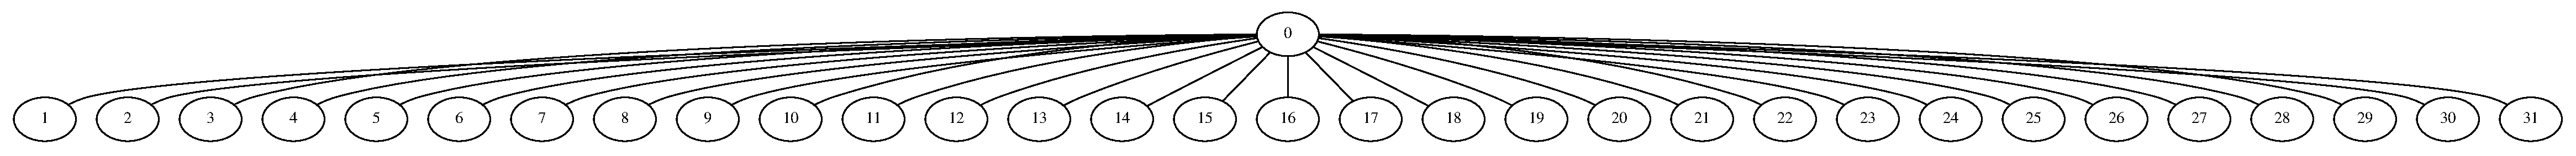
\includegraphics[scale=0.15]{tree-flat}}\\ flat\\
  \vspace{0.5cm}
  \fbox{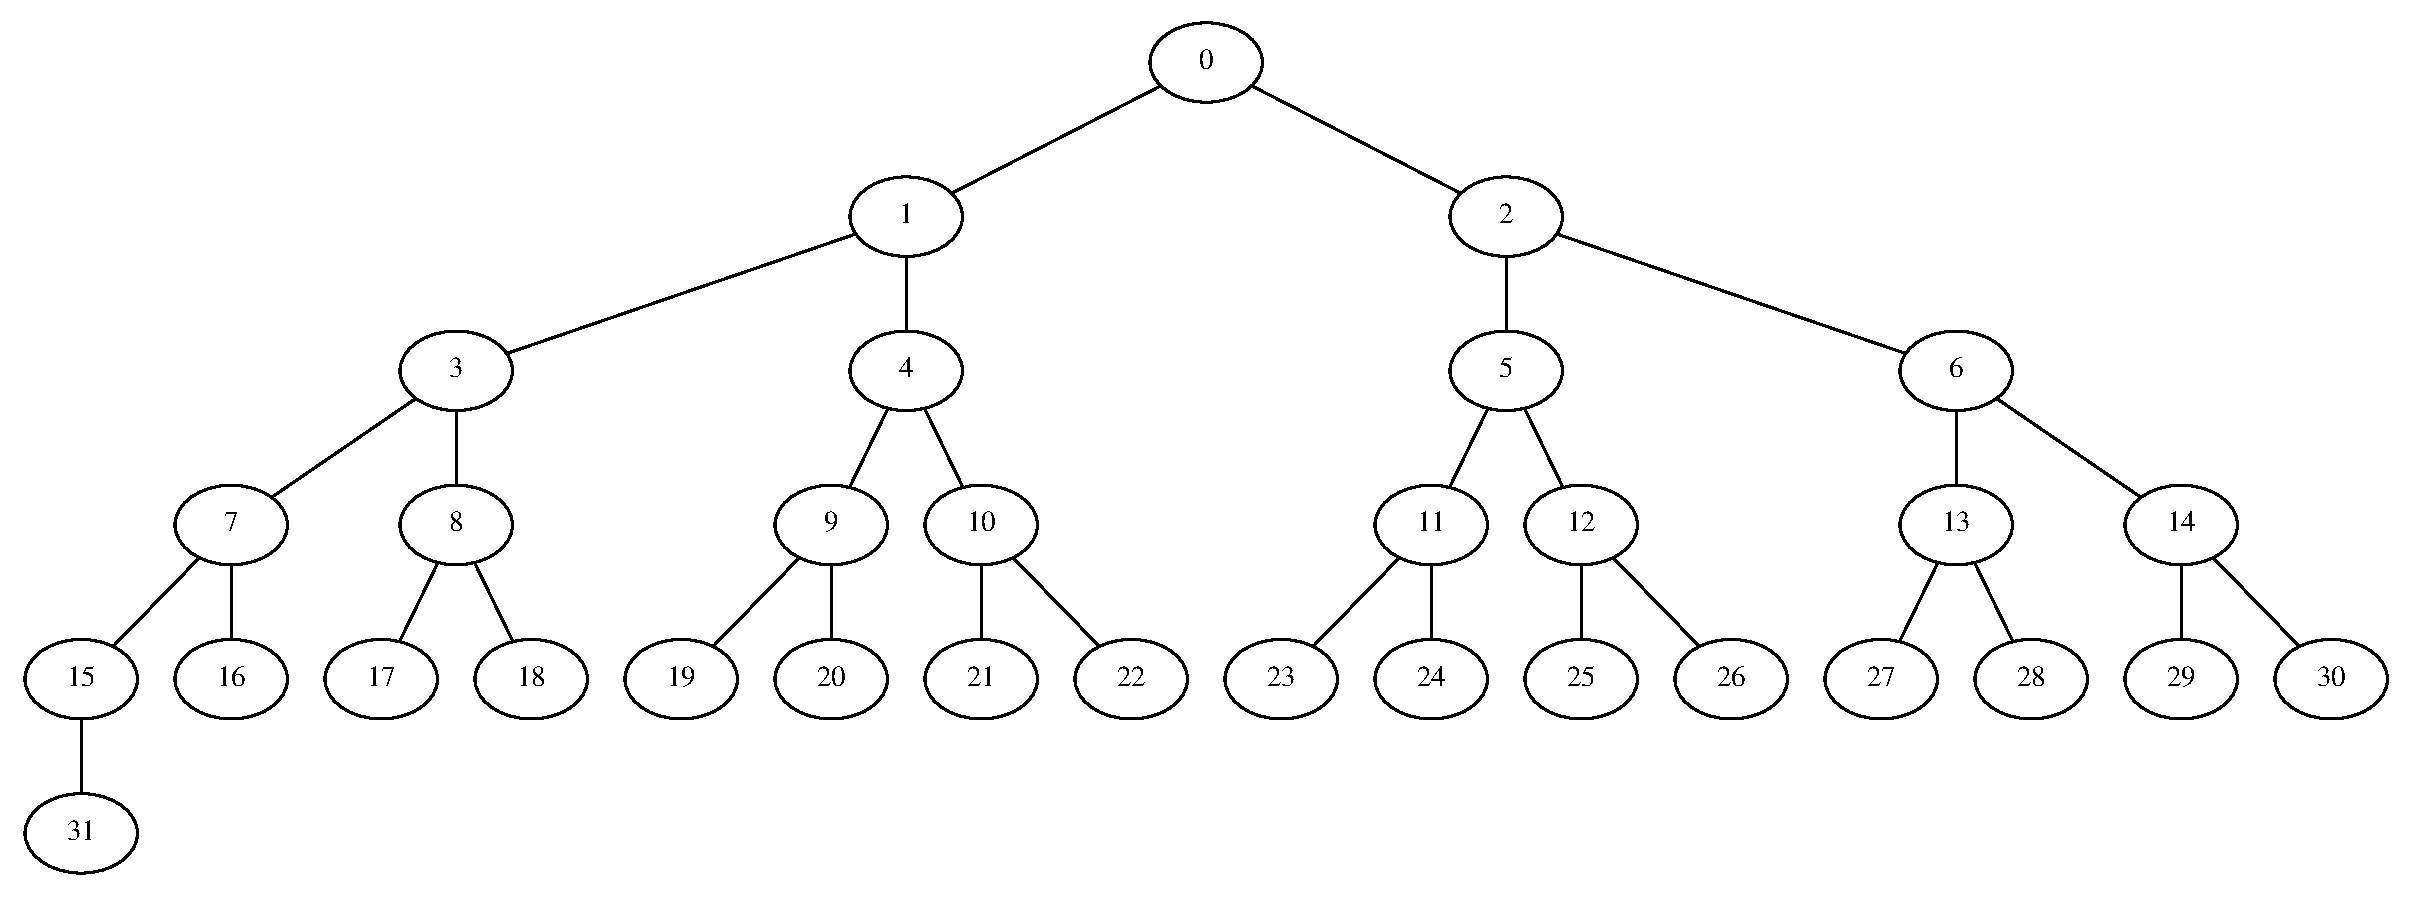
\includegraphics[scale=0.3]{tree-binary}}\\ binary\\
  \vspace{0.5cm}
  \fbox{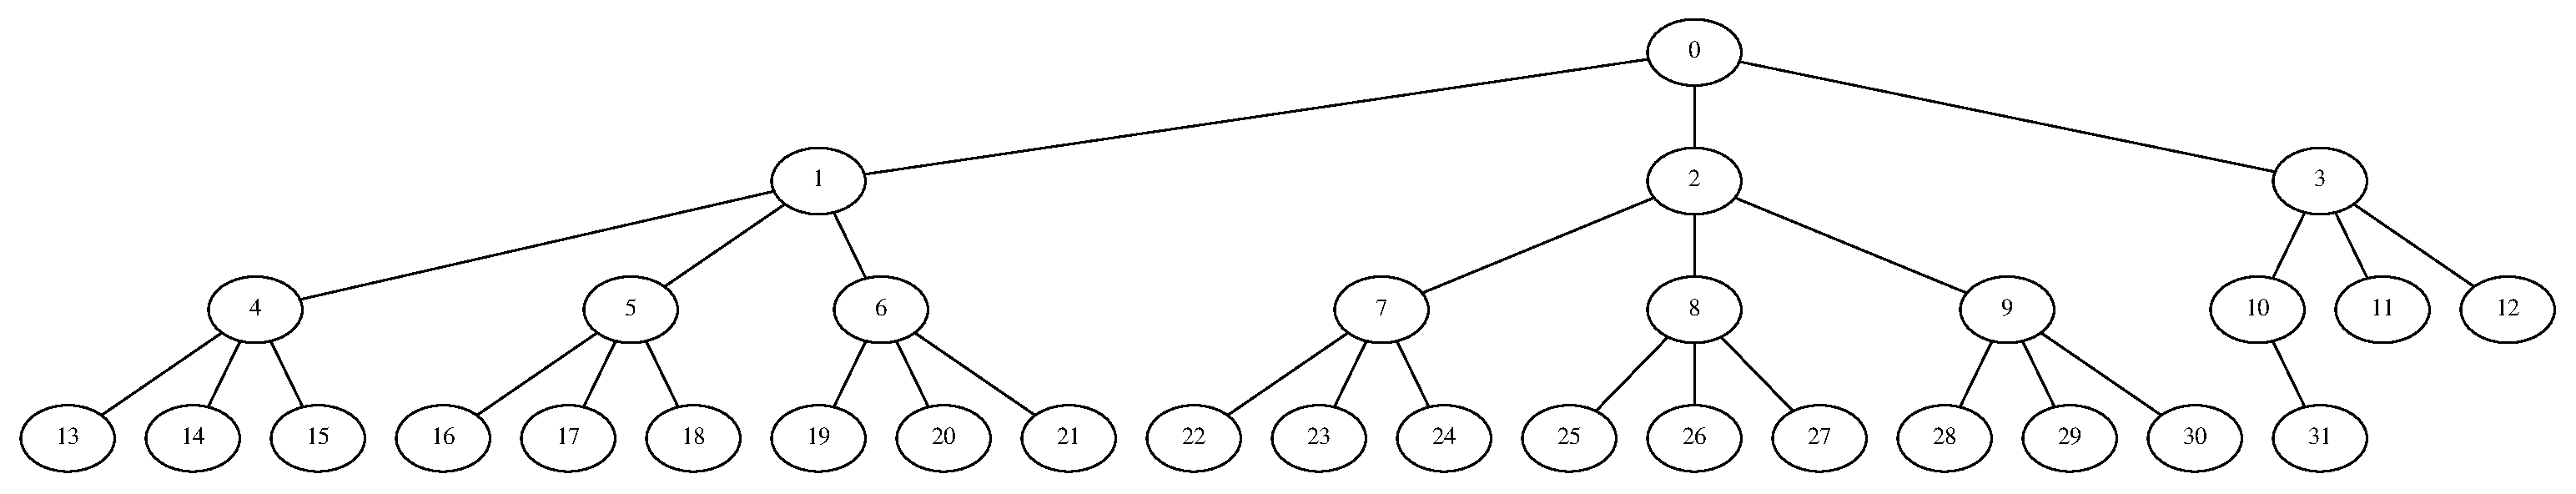
\includegraphics[scale=0.2]{tree-trinary}}\\ trinary\\
  \vspace{0.5cm}
  \fbox{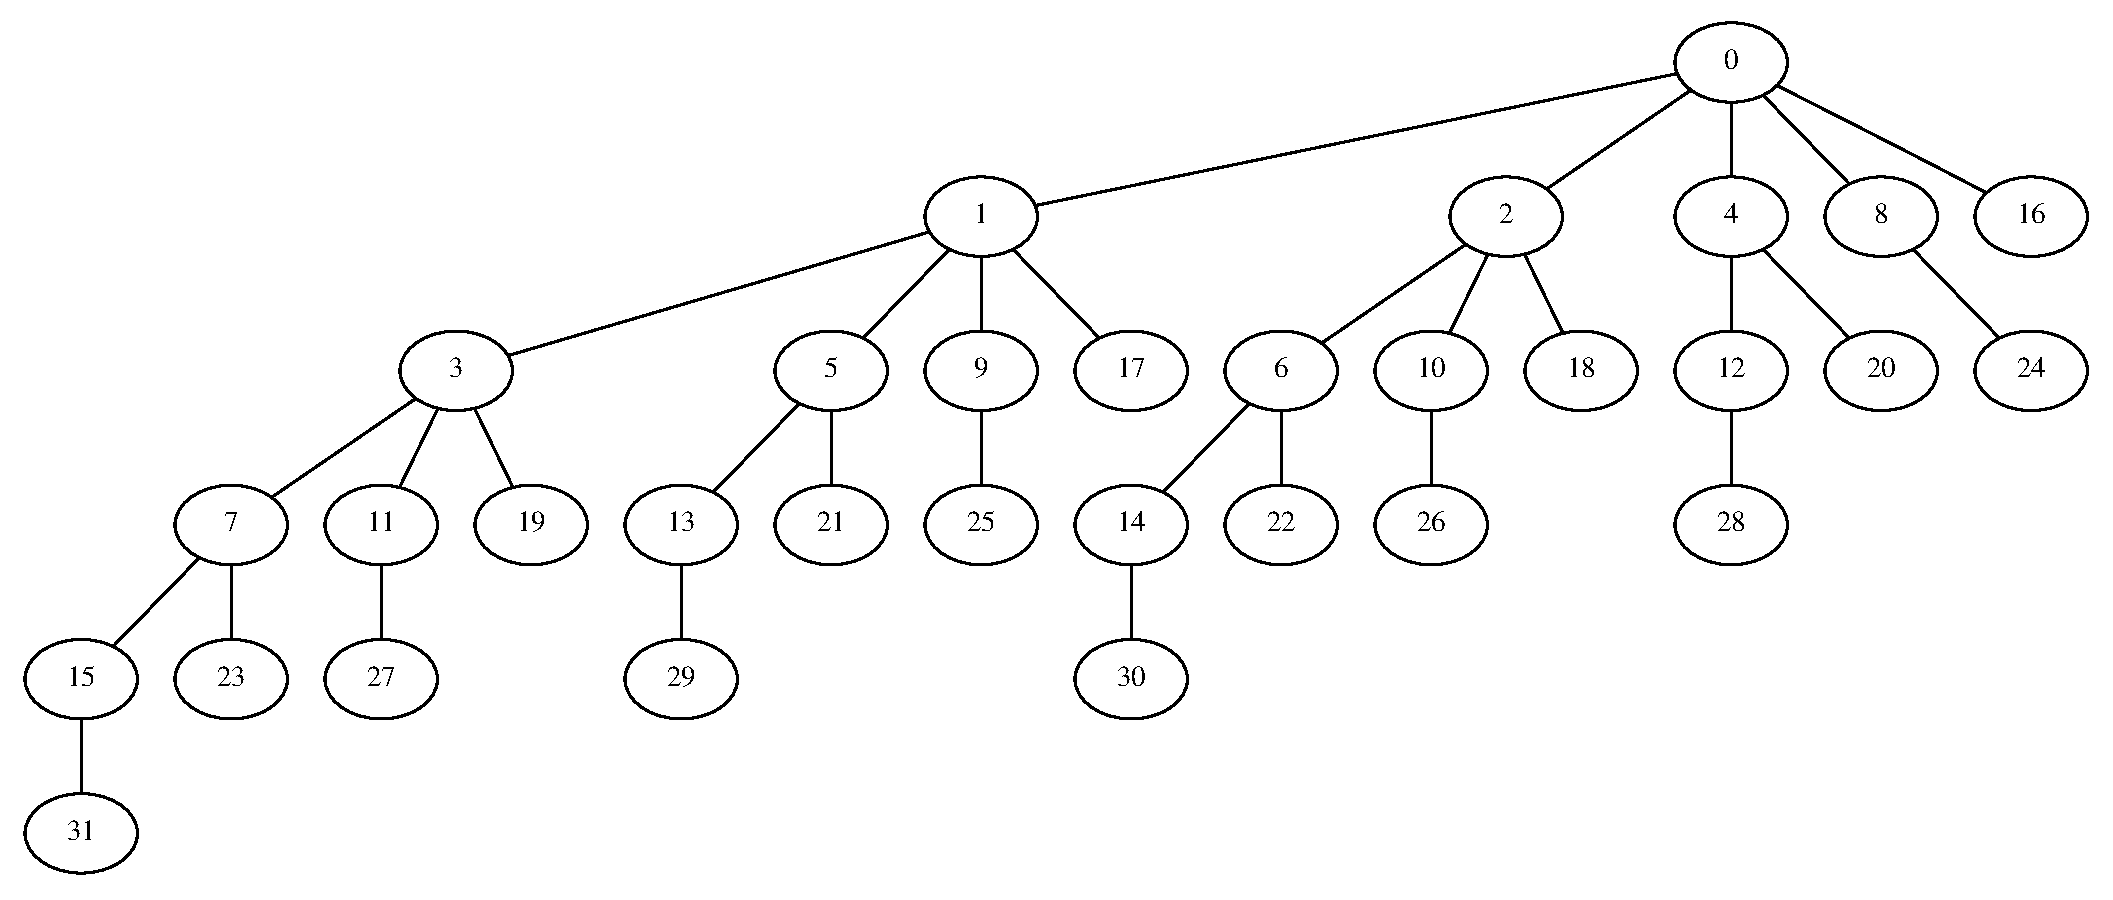
\includegraphics[scale=0.3]{tree-binomial}}\\ binomial\\
\end{minipage}

\caption{The cmbd daemon is built to function without knowledge of its
interconnection topology, except that it is a tree rooted at rank 0.
At launch time it is told its rank, its parent rank, and the total number
of ranks in the session.
Various topologies can be tested by using different functions in the
{\em pepe} lua configuration script to calculate the parent rank from
the node rank.
The topologies depicted above were tested to 100 nodes (32 nodes shown).}
\label{fig:treetop}
\end{figure}


\begin{figure}
\centering
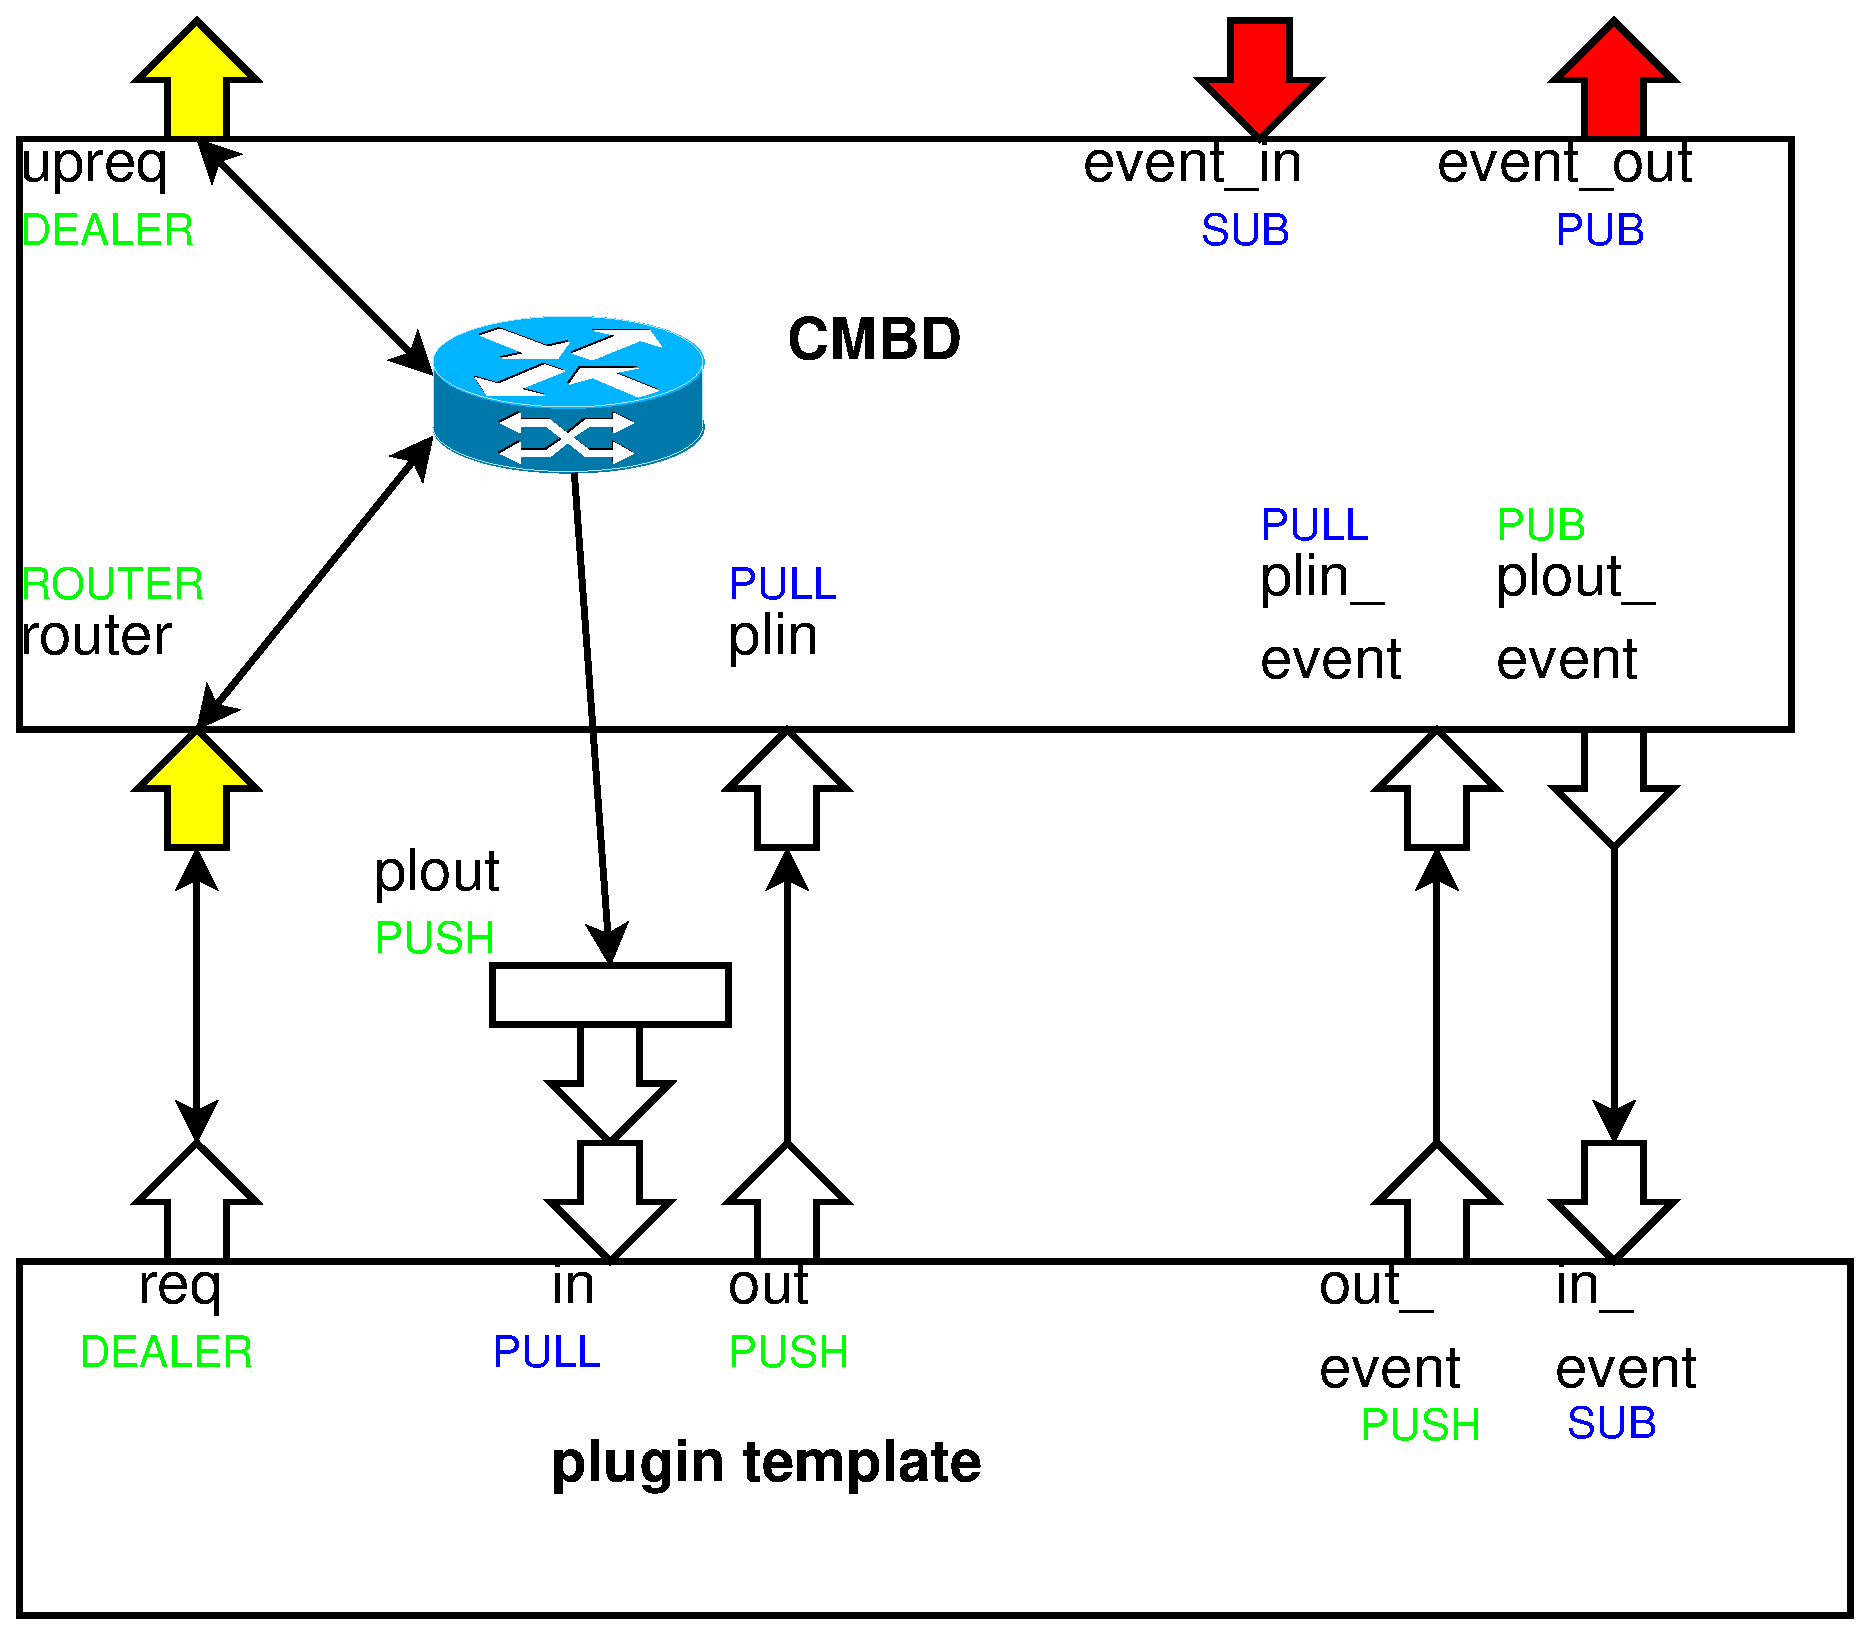
\includegraphics[scale=0.30]{zmq-broker2.eps}
\caption{Broker internal architecture.
The event pub/sub architecture remains basically unchanged from the
previous prototype.  The router socket allows plugins to make requests
that are routed to other plugins by internal routing engine (blue),
and then the \zMQ\ extended REQ-REP message envelopes allow replies
to retrace the same route as the request to the original sender.
The router socket is now used also for the reduction network.  This
architecture allows services to be located anywhere in the hierarchy
transparent to applications.  The routing engine sends requests upstream
if they cannot be matched to a local plugin.}
\label{fig:cmbint2}
\end{figure}

\begin{table}
\centering
\begin{tabular}{|p{0.7cm}p{5cm}|p{9cm}|}\hline
\multicolumn{2}{|l|}{\textbf{Function}}
  & \textbf{Description} \\
\hline
{\tt cmb\_t} & {\tt cmb\_init (void)}
  & Create a {\em cmb\_t} context for communicating with the broker.\\
{\tt void} & {\tt cmb\_fini (cmb\_t c)}
  & Destroy a {\em cmb\_t} context.\\
\hline
{\tt int} & {\tt cmb\_ping (cmb\_t c, int seq, int padding, char **tp)}
  & Send a ping message to the broker's internal bus and wait for it
    to be echoed back.  {\em padding} bytes of payload will be added to
    the message.
    On success, returns $0$; on failure, returns $-1$ with errno set.\\
\hline
{\tt int} & {\tt cmb\_snoop (cmb\_t c, bool enable)}
  & Subscribe/unsubscribe to all messages on the snoop socket.
    On success, returns $0$; on failure, returns $-1$ with errno set.\\
{\tt int} & {\tt cmb\_snoop\_one (cmb\_t c)}
  & Print one snoop message.
    On success, returns $0$; on failure, returns $-1$ with errno set.\\
\hline
{\tt int} & {\tt cmb\_event\_subscribe (cmb\_t c, char *sub)}
  & Subscribe to event messages.  May be called multiple times.
    Same rules as \zMQ subscriptions.
    On success, returns $0$; on failure, returns $-1$ with errno set.\\
{\tt int} & {\tt cmb\_event\_unsubscribe (cmb\_t c, char *sub)}
  & Unsubscribe to event messages.  May be called multiple times.
    Same rules as \zMQ subscriptions.
    On success, returns $0$; on failure, returns $-1$ with errno set.\\
{\tt char *} & {\tt cmb\_event\_recv (cmb\_t c)}
  & Receive one simple event message.
    On success, returns event string (caller must free);
    on failure, returns NULL with errno set.\\
{\tt int} & {\tt cmb\_event\_send (cmb\_t c, char *event)}
  & Send one simple event message.
    On success, returns $0$; on failure, returns $-1$ with errno set.\\
\hline
{\tt int}
  & {\tt cmb\_barrier (cmb\_t c, char {*name}, int nprocs)}
  & Execute barrier {\em name}.  The call blocks until {\em nprocs}
    processes have entered the barrier.  
    All processes entering a given barrier must call this function with
    identical arguments.
    On success, returns $0$; on failure, returns $-1$ with errno set.\\
\hline
{\tt int}
  & {\tt cmb\_kvs\_put (cmb\_t c, char {*key}, char {*val})}
  & Set {\em key} to {\em val} in the job-wide key-value store.
    If the key already has a value, it is overwritten.
    Errors resulting from the actual KVS transaction are not reported
    until the next {\em cmb\_kvs\_commit} call.
    On success, returns $0$; on failure, returns $-1$ with errno set.\\
{\tt {char*}}
  & {\tt cmb\_kvs\_get (cmb\_t c, char {*key})}
  & Retrieve the value of {\em key} from the job-wide key-value store.
    On success, returns a copy of value which the caller must free;
    on failure, returns NULL with errno set.\\
{\tt int}
  & {\tt cmb\_kvs\_commit (cmb\_t c, int *errcount, int *putcount)}
  & Block until the job-wide key-value store has completed all transactions
    originating on the local node.  {\em putcount} will contain the number
    of {\em cmb\_kvs\_put} calls executed by this context since the last commit.
    {\em errcount} will contian the number of failed puts since the last commit.
    On success, returns $0$; on failure, returns $-1$ with errno set.\\
\hline
\end{tabular}
\caption{Public interfaces exported by the broker, take 2.}
\label{tab:cmbapi2}
\end{table}
